\section{Procedure}

\begin{figure*}[th]   
    \noindent
        \centering
            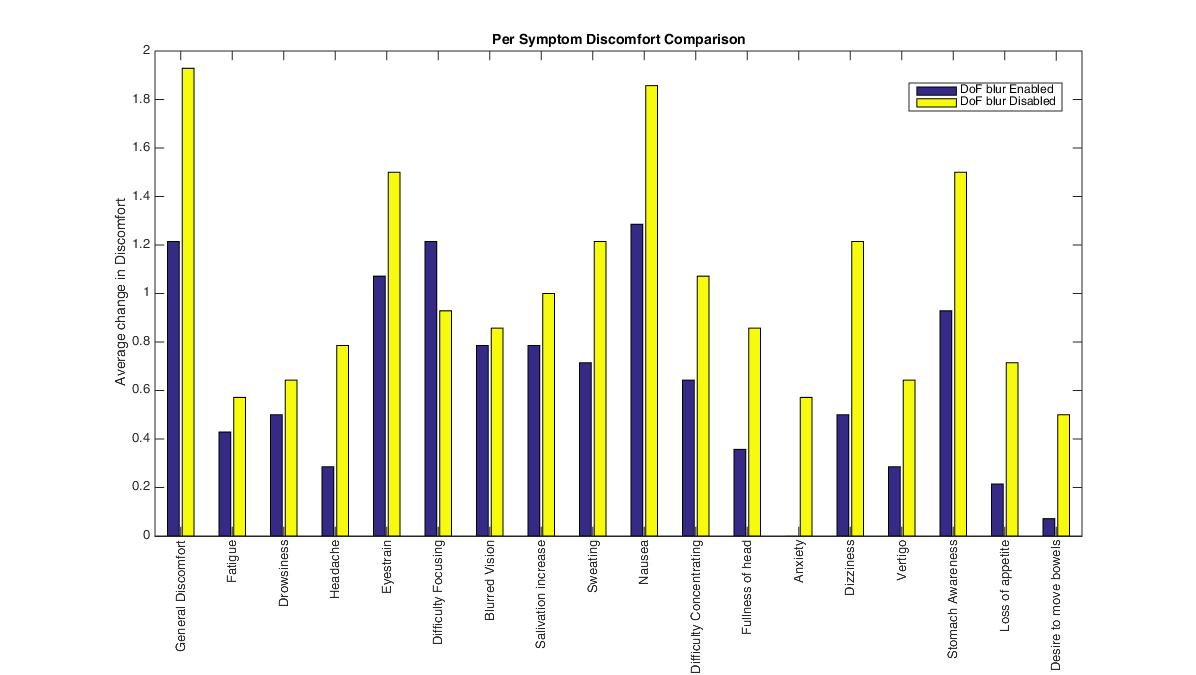
\includegraphics[width=\textwidth]{images/perSymptom.jpg}
            \caption{A comparison between average of participant responses with DoF blur enabled and disabled.}
            \label{fig:sicknessBreakdown}
\end{figure*}


Participants involved in the study were invited to two sessions on sequential working days. In the first session, the participant was shown the two scenes in a random order, with DoF blur applied to one randomly chosen scene. In the second session, the DoF blur was applied to the other scene, and the ordering of the scenes was reversed. The number of participants whose first session had DoF blur enabled was equal to the number of participants whose first session had DoF blur disabled.\\
% minor rearrange needed to fit

For this study, we used a SSQ consisting of 18 questions. For each question, the participant is verbally asked as to their current experience of a symptom, using a 5 point Likert scale (ranging from \say{None}, indicating no presence of that particular symptom, to \say{Severe}, indicating severe or traumatic presence). The SSQ responses resulted in a 18 part measurement of subjective discomfort across specific symptoms, as well as a \textbf{\textit{total sickness measure}} derived from the sum of user responses, multiplied by weights used by~\cite{kennedy93}.\\

At the beginning of each session, participants were asked to complete a SSQ. They then put on the Oculus and adjusted its physical settings to be comfortable. Participants with glasses were given the option to wear them inside the Oculus if they could fit, otherwise the appropriate lenses were put into the Oculus to compensate.\\

The nature of the control scheme was then explained to each participant. They were given a minute to get used to how the controls worked, and then explored whichever scene had been randomly chosen for 15 minutes. A SSQ was then verbally completed. Participants were asked to close their eyes, and were relocated to the other scene, which they then explored for another 15 minutes before completing the third SSQ and taking off the Oculus. They were then asked to relax and wait 15 minutes, before completing a final SSQ. Each SSQ was administered verbally.\\

